\chapter{Installation}\label{installation}

In this chapter we will install and run the Python interpreter in your local computer.

\section{Installing on Windows}

\begin{enumerate}

\item Download the latest Python 3 release for Windows on \url{https://www.python.org/downloads/windows/} and execute the installer. At the time of writing, this is Python 3.6.4.

\item Make sure that the "Install launcher for all users" and "Add Python to PATH" settings are selected and choose "Customize installation".

\begin{figure}[H]
	\centering
  	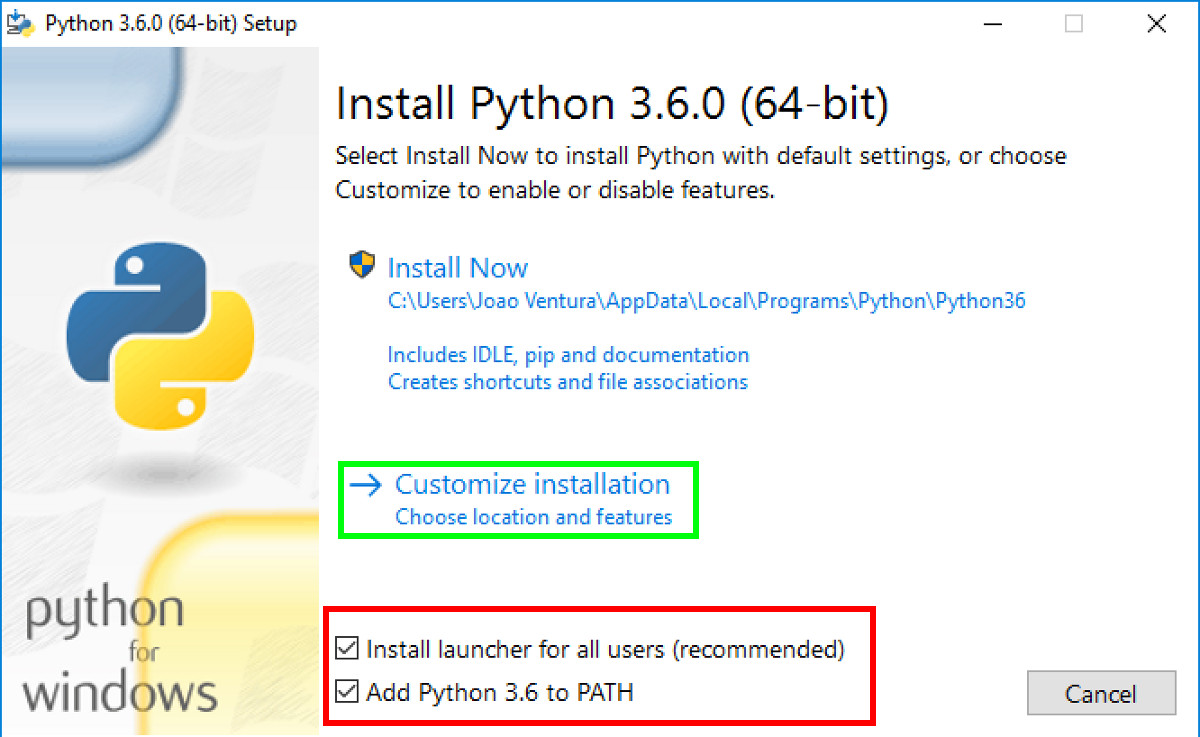
\includegraphics[width=0.6\textwidth]{images/python_windows.jpg}
\end{figure}

\item In the next screen "Optional Features", you can install everything, but it is essential to install "pip" and "pylauncher (for all users)". Pip is the Python package manager that allows you to install several Python packages and libraries.

\item In the Advanced Options, make sure that you select "Add Python to environment variables". Also, I suggest that you change the install location to something like C:{\textbackslash}Python36{\textbackslash} as it will be easier for you to find the Python installation if something goes wrong.

\begin{figure}[H]
	\centering
  	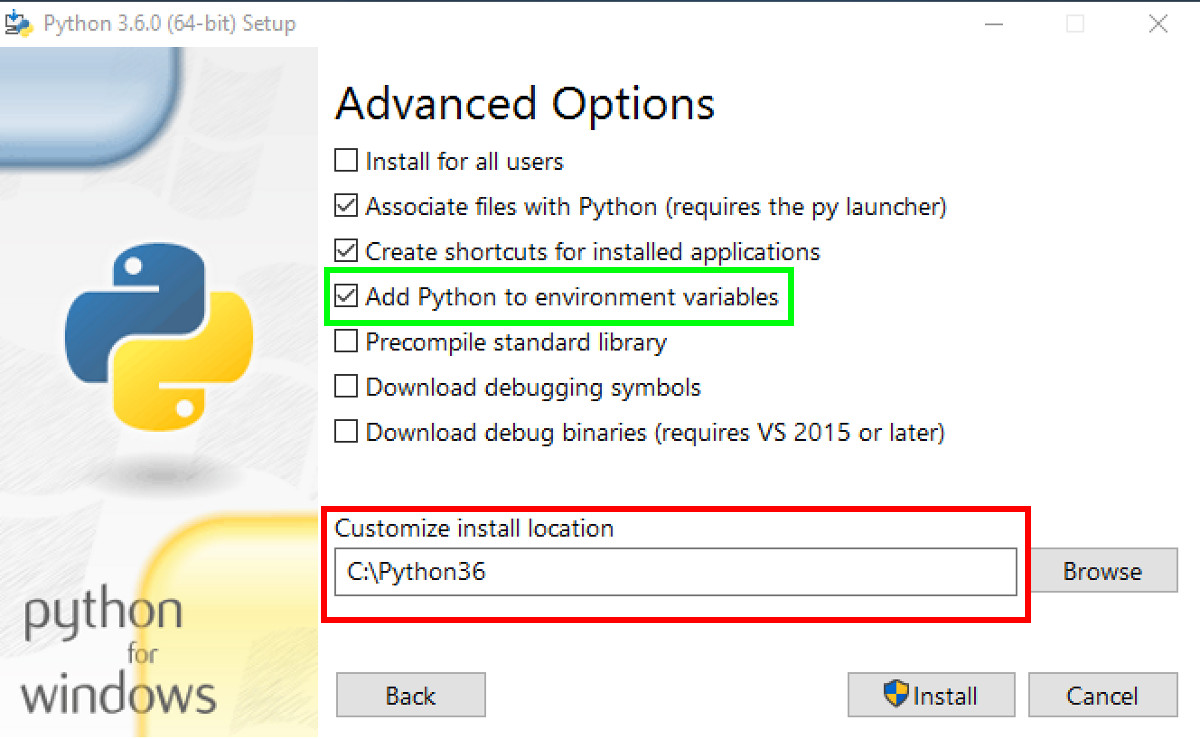
\includegraphics[width=0.6\textwidth]{images/python_windows2.jpg}
\end{figure}

\item Finally, allow Python to use more than 260 characters on the file system by selecting "Disable path length limit" and close the installation dialog.

\begin{figure}[H]
	\centering
  	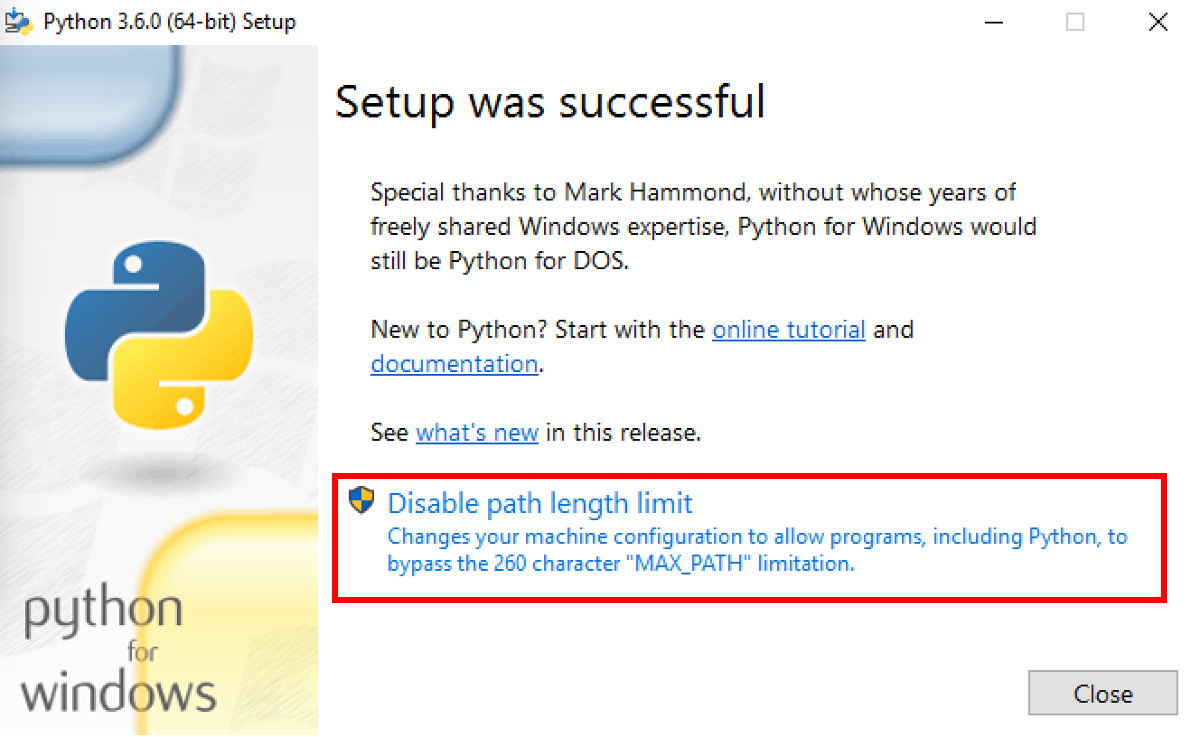
\includegraphics[width=0.6\textwidth]{images/python_windows3.jpg}
\end{figure}

\item Now, open the command line (cmd) and execute "python" or "python3". If everything was correctly installed, you should see the Python REPL. The REPL (from Read, Evaluate, Print and Loop) is a environment that you can use to program small snippets of Python code. Execute \textit{exit()} to exit.

\begin{figure}[H]
	\centering
  	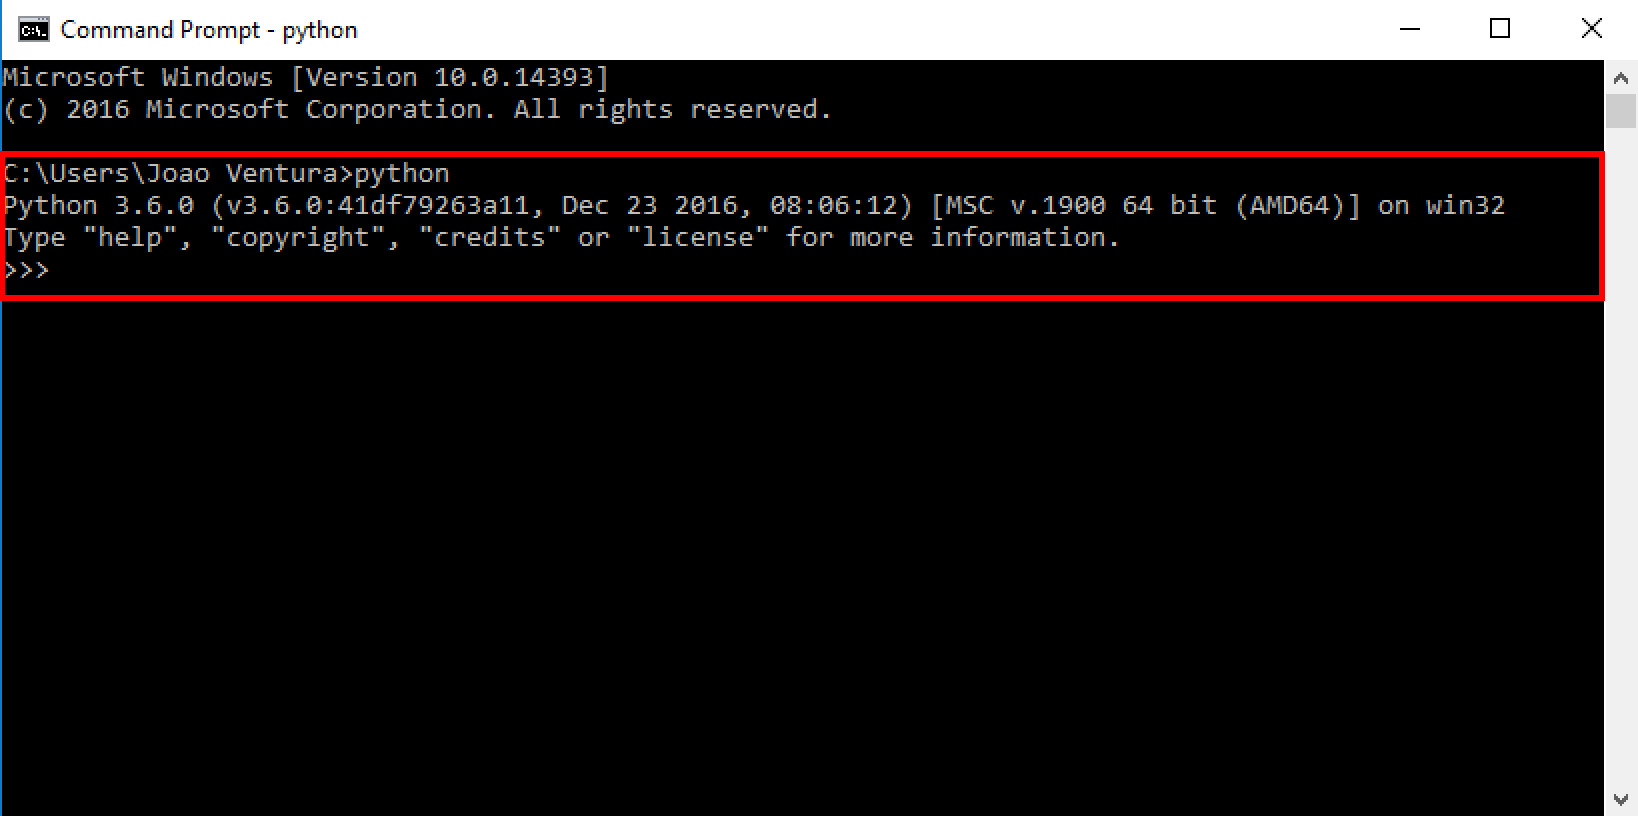
\includegraphics[width=0.62\textwidth]{images/python_windows4.jpg}
\end{figure}

\end{enumerate}

\section{Installing on macOS}

You can download the latest macOS binary releases from \url{https://www.python.org/downloads/mac-osx/}. Make sure you download the latest Python 3 release (3.6.4 at the time of writing). You can also use Homebrew, a package manager for macOS (\url{https://brew.sh/}). To install the latest Python 3 release with Homebrew, just do "\texttt{brew install python3}" on your terminal. Another option is to use MacPorts package manager (\url{https://www.macports.org/}) and command "\texttt{port install python36}".  


\begin{figure}[H]
	\centering
  	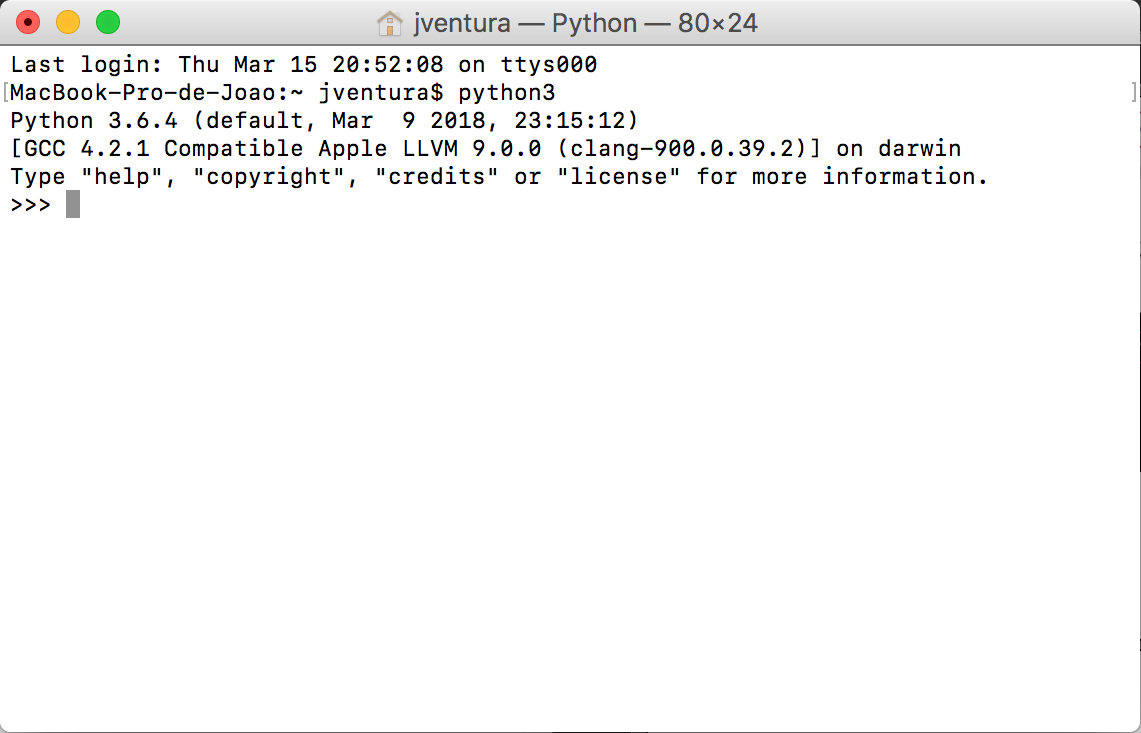
\includegraphics[width=0.62\textwidth]{images/python_macos.png}
\end{figure}

Finally, open the terminal, execute $python3$ and you should see the Python REPL as above. Press Ctrl+D or write $exit()$ to leave the REPL.

\section{Installing on Linux}

For Linux, you can download the latest Python 3 binary releases from \url{https://www.python.org/downloads/linux/} or use your package manager to install it. To make sure you have Python 3 installed on your system, run $python3$ in your terminal.

\begin{figure}[H]
	\centering
  	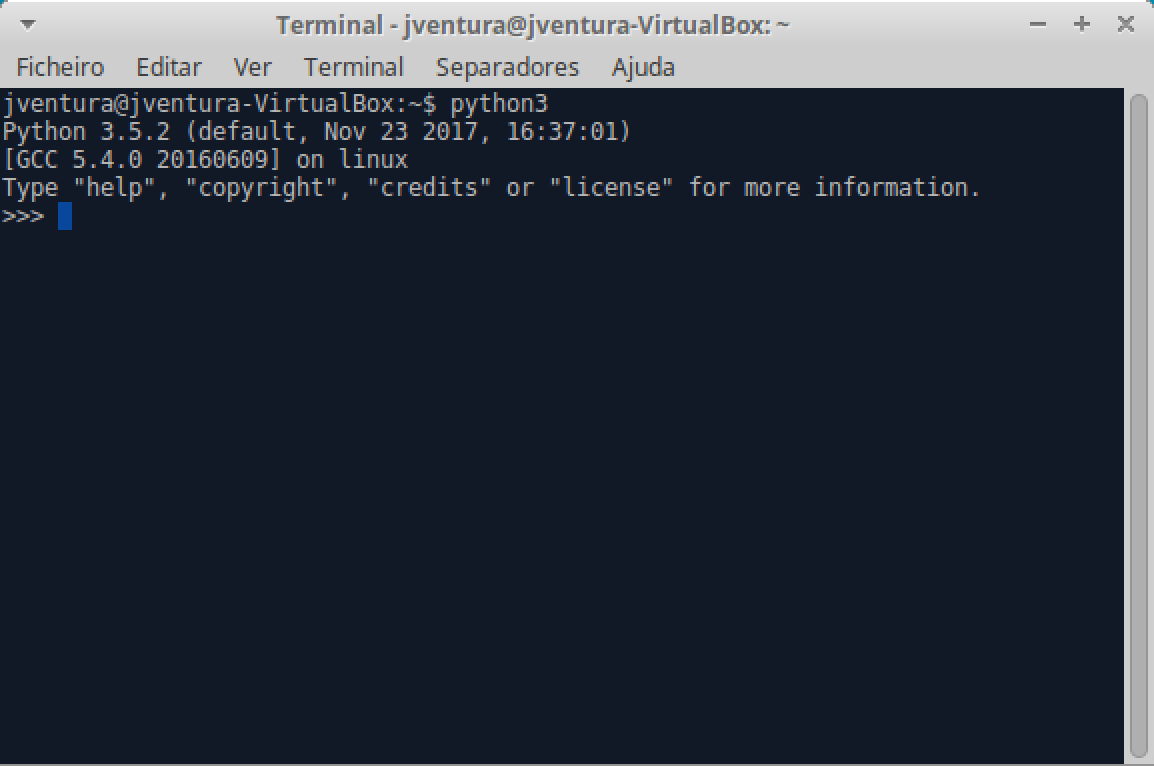
\includegraphics[width=0.62\textwidth]{images/python_linux.png}
\end{figure}

Finally, open the terminal, execute $python3$ and you should see the Python REPL as above. Press Ctrl+D or write $exit()$ to leave the REPL.
